\section{Information Overload}

Information overload conveys the act of receiving \emph{too much information}. 
The problem is apparent in situations where decisional accuracy turns from improving with more information, 
to being hindered by too much irrelevant data \cite[p13]{Bjorkoy2010d}. 
This is a widespread phenomenon, with as many definitions as there are fields experiencing the problem. 
Examples include \emph{sensory overload}, \emph{cognitive overload} and \emph{information anxiety} \cite[p2]{Eppler2004}.
Two common tasks quickly become difficult when this happens:

\begin{enumerate*}
  \item Consumption of relevant content is hindered by too much irrelevant noise.
  \item Discovering new and interesting content is difficult because of too much information.
\end{enumerate*}

\noindent
Finding contemporary examples is not difficult:

\begin{itemize*}
  \item Missing important news articles that get drowned out by irrelevant content.
  \item Forgetting to reply to an email as new messages keep arriving.
  \item Consuming sub-par entertainment because the most relevant is never discovered.
  \item Reformulating search queries because the results include irrelevant items.
  \item Browse through much information to find what one is actually looking for.
\end{itemize*}

Information overload is often likened to a \emph{paradox of choice}, as there may be no problem acquiring the relevant information, 
but rather identifying this information once acquired. As put by \cite[p6]{Edmunds2000}: 
\emph{``The paradox --- a surfeit of information and a paucity of useful information.''}
While normal cases of such overload typically result in feelings of being overwhelmed and out of control, 
\citet[p5]{Bawden2008} points to studies linking extreme cases to various psychological conditions 
related to stressful situations, lost attention span, increased distraction and general impatience.

\cite{Kirsh2000} argues that 
\emph{``the psychological effort of making hard decisions about \emph{pushed} information is the first cause of cognitive overload.''} 
According to \citeauthor{Kirsh2000}, there will never be a fully satisfiable solution to the problem of overabundant information, 
but that optimal environments can be designed,
in order to increase productivity and reduce the level of stress.
This is achieved through careful consideration of each user's needs. 
To solve the problems of information overload, 
applications must be able to individually adapt themselves to each user. 

An insightful perspective on information overload comes from the study of \emph{attention economy}. 
In this context human attention is seen a scarce commodity, offset by how much irrelevant noise is present at any given time. 
\citet[p1]{Davenport2001} defines attention as \emph{``[...] focused mental engagement on a particular item of information. 
Items come into our awareness, we attend to a particular item, and then we decide whether to act''.} 
To evade information overload means maximising the available attention, allowing more focus on the most important items in each situation.

\begin{wrapfigure}{rt}{0.5\textwidth}
  \vspace{-20pt}
  \begin{center}
    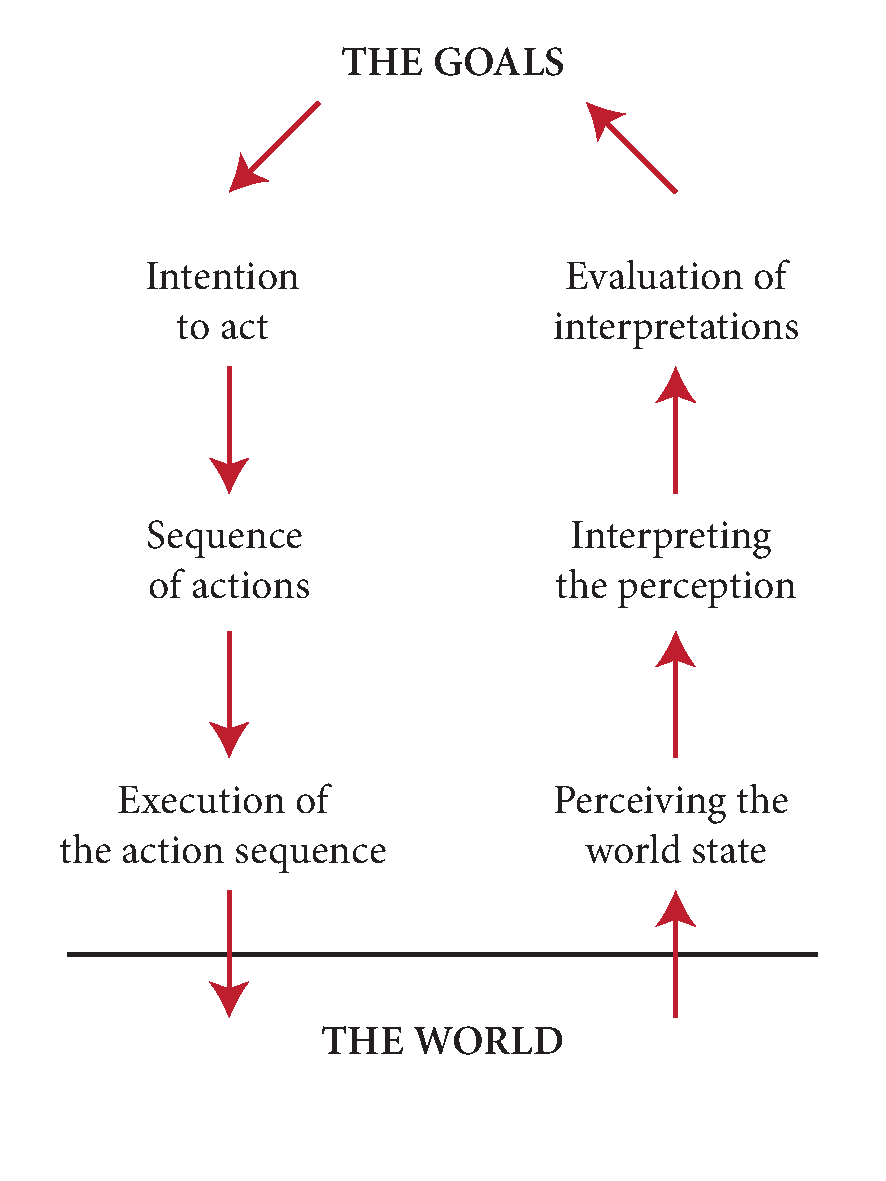
\includegraphics[width=0.5\textwidth]{../graphics/seven-stages.pdf}
    \vspace{-20pt}
    \caption[The Seven Stages of Action]{Stages of Action}
  \end{center}
  \label{fig:seven-stages}
  \vspace{-20pt}
\end{wrapfigure}

Conceptual models used in interaction design can also help us see when and where information overload interferes with a user's experience. 
\cite{Norman1988} advocates a model called \emph{the seven stages of action}, 
that describes how each user goes through several states while using a system
(see Figure \ref{fig:seven-stages}, adapted from \citeauthor{Norman1988}). 
First, the user forms a goal and an intention to act. The user then performs a sequence of actions on the world (the interface)
 meant to align the perceived world and the goals. After performing a set of actions, the new world state is evaluated and perceived. 
At last, the user evaluates the perception and interpretation of the world in accordance with the original goal.

As apparent from this model, information overload can interfere both before and after any action is taken. 
For example, if the application presents too much content, or presents content in a confusing manner, 
it can be difficult for the user to identify which actions that would help achieve the current goal. 
Likewise, after actions are taken, the new world state can suffer the same shortcomings of overwhelming scope or lack of presentations, 
leading to information overload. 
This precludes the user from properly evaluating the resulting application state. 

In short, an application interface can fail both before and after a user tries to interact with it.
Information overload happens throughout the interaction process.


\subsection{Online Overload}

The Web is a common source of information overload, 
and a good example of how and why the problem occurs.
Online information overload is especially pervasive when considering \emph{content aggregating websites}:
Web sites that combine information from multiple other sites and sources. 
Online information retrieval systems (search engines) are in category, as are
online newspapers, feed readers and portal sites.

The wealth and scope of data on the Web are natural culprits of online overload, 
as well as the varying qualities of websites publishing the information. 
However, the problem is also a result of the fundamental observed structure of the Web.
Graph theory presents applicable models that characterize how people navigate between websites, 
and show how content aggregators form important hubs in the network. 
These models give a theoretical foundation for why information overload occurs on the Web.

In the Web graph, nodes correspond to websites and
directed edges between nodes are links from one page to another. The \emph{degree} of a node is defined as its number of edges.
This graph has the properties of a \emph{small-world network} (\citep{Newman2000}, \citep[p2]{Huang2005}), 
a type of random graph, where most nodes are not neighbors, but most nodes are reachable through a small number of edges (See Figure \ref{fig:swn}). 
This is because of important random shortcuts differentiating the graph from a regular lattice. 
The graph is not  random, but neither is it completely regular.
As described by \citet[p37]{Barabasi2003}, the average number of outbound links from a web page is around 7.
From the first page, we can reach 7 other pages. From the second, 49 documents can be reached. 
After 19 links have been traversed, about $10^{16}$ pages can be reached (which is more than the actual number of existing web pages, since loops will form in the graph).

\begin{figure}[t]
  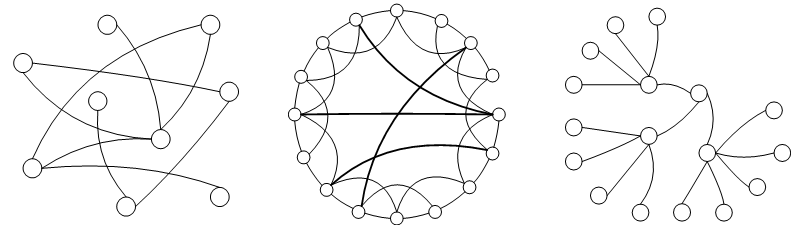
\includegraphics[width=\textwidth]{../graphics/graphs}
  \caption[Examples of Complex Networks]{
    Complex Networks,
    from the left: A \emph{random} network, a \emph{small-world} network and a \emph{scale-free} network 
    (which is a type of  small-world network). Figure adapted from \citep[p2]{Huang2005}.} 
  \label{fig:swn}
\end{figure}

The high degree of the Web graph would suggest that finding an optimal path to your desired page is quite difficult. 
Yet, while it is true that finding the \emph{optimal path} is hard, finding \emph{a good path} is not that big a challenge. 
When people browse the Web, links are not followed blindly --- 
we use numerous heuristics to evaluate each link, often resulting in quite a good path to where we want to go. 
So why is the Web still quite challenging to navigate?

As discovered by \cite{Albert1999}, the Web also exhibits properties of a \emph{Scale-Free Network} (\smallcaps{SFN}). 
They found that in some natural observed networks, there exists a small number of nodes with an extremely high degree. 
This is also true on the Web --- some websites have a huge number of outbound links. 
For comparison, while a random network is similar to a national highway system, with a regular number of links between major cities, scale-free networks are more like an air traffic system, with central hubs connecting many less active airports \citep[p71]{Barabasi2003}.

These highly connected nodes, called \emph{hubs}, are not found in small-world networks or random graphs. As demonstrated by the presence of hubs, the degree distribution of a scale-free network follows a power law, 
$P(k) \sim k^{-\gamma}$, 
where $P(k)$ is the probability of a node having k connections and $\gamma$ is a constant dependent on the type of network, typically in the range $2 < \gamma < 3$. 
Since the Web has directed edges,
we have two power laws:
$P_{in}(k) \sim k^{-\gamma_{in}}$ and 
$P_{out}(k) \sim k^{-\gamma_{out}}$.

\cite{Albert1999} describes a number of studies placing the $\gamma$ values for the Web in the $[2,3]$ range, 
with $\gamma_{out}$ being slightly higher than $\gamma_{in}$. 
Both these probabilities exhibit power tails (or long tails). 
A few important nodes have a huge number of inbound and outbound links, i.e. the hubs. 

\citet[p86]{Barabasi2003} proposed that hubs emerge in a scale-free networks because of two factors:
\emph{(1) Growth:} Nodes are added to the network one by one, for example when new websites are added to the Internet.
\emph{(2) Preferential attachment:} When new nodes are created, they connect to existing nodes. The probability that the new node will connect to an existing node is proportional to the number of links the existing node has. Older, more established and central nodes are preferred neighbors.

This is called the Barab\'{a}si-Albert model \citep{Albert1999}. 
The probability for a new node connecting to an existing node is given by $\prod k_i$, 
where $k_i$ is the number of links pointing to node $i$, in the following equation: 

\begin{equation*}
  \prod_{i} k_i  = \frac{k_i}{\sum_{j}^N k_j}.
\end{equation*} 

Search engines, social link aggregators, news portals, et cetera are all hubs of the Internet, emerging from the preferential 
link attachment of newly created nodes, that make navigating the Web less easy as it might appear.
What does seem clear is that these content aggregating hubs are prime candidates for overwhelming their users with information. 

The fundamental observed structure of the Web creates the need for information brokers that link the net together, 
and the need for techniques to display a lot of data --- adapted to each user and each item.
In other words, we need user modeling, that can predict how relevant each item will be for each user.


 
\subsection{Interface Autonomy}

\begin{figure}[t]
  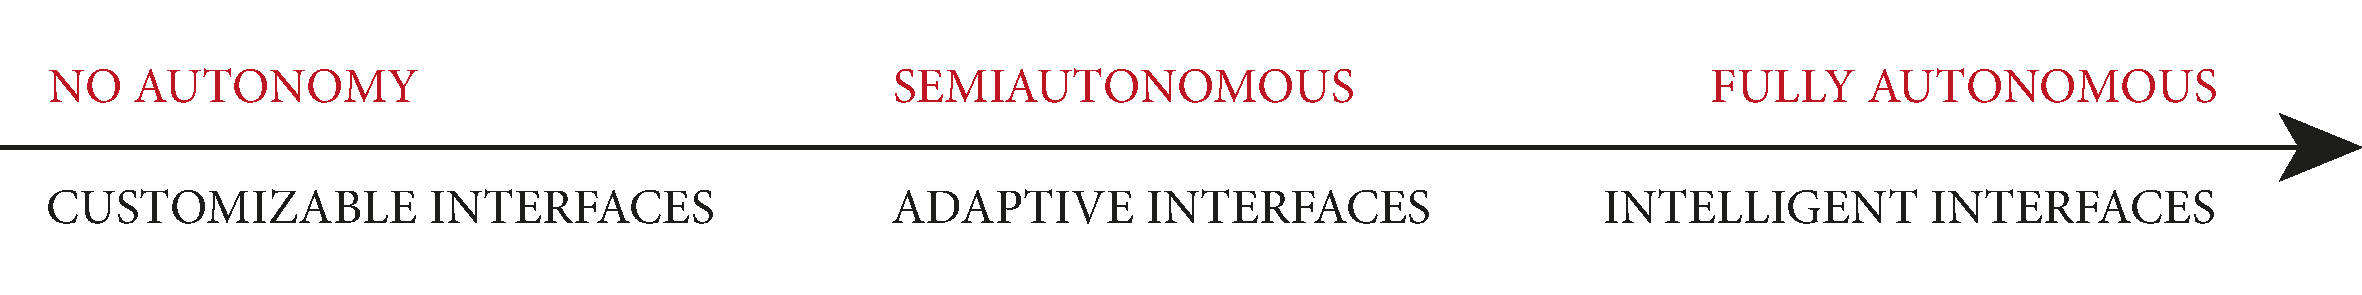
\includegraphics[width=\textwidth]{../graphics/autonomy.pdf}
  \caption[Levels of Interface Autonomy]{
    Levels of Interface Autonomy:
    Interfaces range from those only customizable by the user, 
    to intelligent systems takes the initiative on their own accord.
  }
  \label{fig:autonomy}
\end{figure}

Using AI to adapt an interface raises important questions with regard to usability, privacy and usefulness.
These questions are rooted in the autonomy expressed by each interface.
An autonomous interface is one that takes initiatives on its own, regardless of whether the user has asked for it \cite[p2]{Lieberman}. 
Naturally, any application that automatically personalizes its content will be autonomous to some degree.

Adaptive interfaces can be classified into increasing order of autonomy (see Figure \ref{fig:autonomy}). 
At the order of least autonomous systems, we have \emph{customizable interfaces}. 
These are interfaces that the user may customize themselves, but that do not take the initiative or change anything without explicit user action. 
For example, an interface might have a settings panel where users can change the order of items in a menu.

At the next level of autonomy, we have \emph{adaptive interfaces} that suggest to the user possible changes or actions that might be beneficial. For example, an email application could suggest which folder an email should be moved to.
At the most autonomous level, \emph{intelligent interfaces} implicitly and automatically customize the interface or content based on passive observation of the user. 
This could for instance entail automatic filing of emails based on content classification and data mining of previous user actions with similar messages.

An application that personalizes content automatically will fall somewhere in the two last categories and present either an adaptive or intelligent interface, 
depending on the extent and transparency of its autonomy.

In this thesis, we are only interested in fully autonomous, intelligent interfaces.
We will create a system that implicitly, and without any effort from each user,
can adapt the content of an application based on previous behavior.
Examples of such implicit user modeling include \cite{Qiu2006}, \cite{Shen2005} and \cite{Carmel2009}.


